\chapter[PROCESSAMENTO DE DADOS]{PROCESSAMENTO DE DADOS}
\label{chapter:data}

A camada de processamento de dados que será proposta para o InterSCity terá
como base a utilização de Big Data, considerada uma das três principais
tecnologias na criação de infraestrutura para cidades inteligentes
\cite{kon2016}. Neste capítulo serão detalhadas duas arquiteturas, Lambda e
Kappa, e o levantamento de possíveis tecnologias a serem usadas nestas
arquiteturas. A Arquitetura Lambda foi decidida como dandidata por ser bem
estabelecida e considerada adequada para o contexto de cidades inteligentes
\cite{kiran2015}, enquanto a Arquitetura Kappa foi decidida como candidata por
ser utilizada por grandes empresas, como a
LinkedIn\footnote{\url{https://www.oreilly.com/ideas/questioning-the-lambda-architecture}}.
É importante ressaltar também que adaptações das arquiteturas serão feitas em
relação a literatura, de modo que fiquem mais adequadas ao contexto de cidades
inteligentes, e mais plausíveis para o estado atual do InterSCity.

\section{ARQUITETURA LAMBDA}

A Arquitetura Lambda é um padrão de projeto para plataformas de processamento
de dados que utilizam tecnologias Big Data \cite{kiran2015}, e surge como um
caminho alternativo a outras arquiteturas mais antigas, como a incremental com
\textit{sharding} \cite{marz2015}. É composta de três camadas: a camada
\textit{batch}\footnote{No decorrer do texto, as camadas da arquitetura Lambda
e outros termos associados não serão traduzidos.}, a camada \textit{serving}; e
a camada \textit{speed} \cite{kiran2015}. Cada uma destas camadas é
implementada utilizando algoritmos e ferramentas específicas, de modo
que certas ferramentas são mais apropriadas em certos contextos.

A \textbf{camada \textit{batch}} é responsável pelo processamento de uma grande
massa de dados, e tem como ponto fraco a alta latência. Em sua execução, ela
cria e gerencia um \textit{master dataset}\footnote{O \textit{master dataset} é um lote
histórico de informação, que, por ser imutável, só possibilita \textbf{anexação}
de informações.}, que, após processados, são disponibilizados em
\textit{batch views}, utilizados pela \textbf{camada \textit{serving}}.
A camada \textit{batch} é então, em sua essência, imutável, de modo que, caso
uma mudança seja necessária, uma abordagem diferente deve ser seguida: o dado
que carece alteração não sofre transformações, permanecendo inalterado, mas um
novo dado com as alterações é inserido no lote \cite{marz2015}.

\newpage
A \textbf{camada \textit{speed}} tem como diferencial o processamento com baixa
latência, que é obtido pelo uso de uma parcela menor da massa de dados\footnote{
A camada \textit{speed} só leva em conta dados que surgiram após a camada
\textit{batch} ter começado seu processamento.}. Outra característica importante
é que esta camada faz uso do processamento \textit{streaming}, que ocorre
quando os dados são processados conforme estão disponíveis. Este tipo de
processamento funciona bem com mecanismos de passagem de mensagem
\cite{marz2015}, e permitem que as consultas feitas levem em conta dados
recentes, ignorados pela camada \textit{batch}. Essa abordagem utilizada
pela camada \textit{speed}, incremental, costuma aceitar também alteração de
dados já utilizados, tornando esta camada mutável, o que força o uso de um
banco de dados que suporte escrita aleatória \cite{marz2015}, aumentando
substancialmente a complexidade desta camada \cite{marz2015}. Por fim, a
camada \textit{speed} condensa seu processamento feito em
\textit{real-time views}, que serão fundidos com os resultados das
\textit{batch views}. Os resultados da camada \textit{speed} são então
dispensados sempre que um \textit{batch} terminar seu processamento
\cite{marz2015}.

\begin{figure}
  \centering
    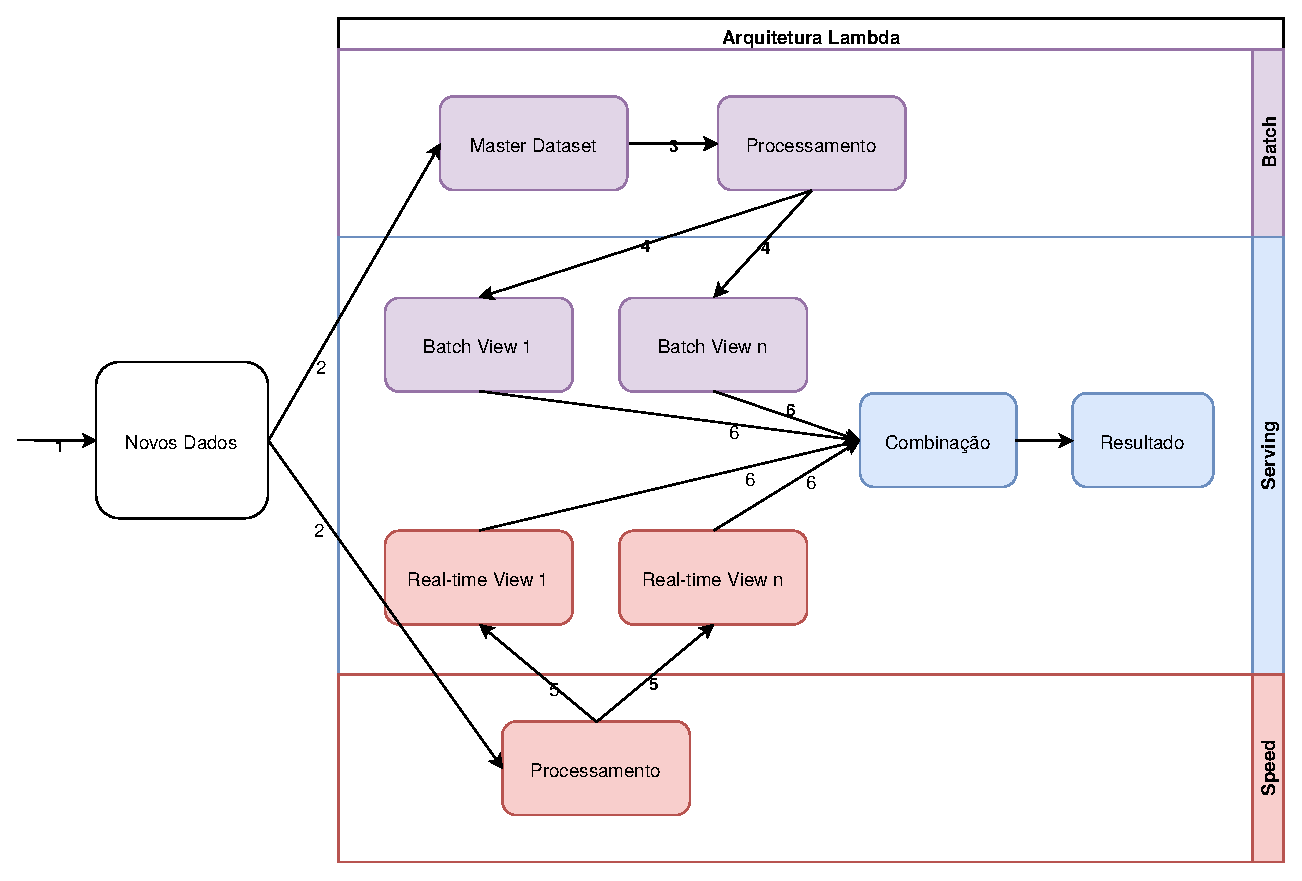
\includegraphics[width=\textwidth]{figuras/lambda-lifecycle.eps}
  \caption{Ciclo de vida na Arquitetura Lambda.}
  \label{fig:lambda-lifecycle}
\end{figure}

Um ciclo de vida típico da Arquitetura Lambda pode ser acompanhado na Figura
\ref{fig:lambda-lifecycle}, e tem seu início com a (i) chegada
de novos dados, que serão então (ii) transmitidos tanto para a camada
\textit{batch} quanto para a camada \textit{speed}. A camada \textit{batch}
(iii) anexa os novos dados, e os processa, (iv) gerando assim
\textit{batch views}, que são enviados para a camada \textit{serving}. O mesmo
dado que foi enviado para a camada \textit{batch}, no passo (i), também foi
enviado para a camada \textit{speed}, onde (v) será processado com menor latência,
por só levar em conta dados recentes, gerando assim \textit{real-time views}. 
Caso uma consulta seja feita, ocorrerá então uma (vi) soma entre os resultados
dos \textit{batch views} e \textit{real-time views}, que é então a resposta
a consulta \cite{marz2015}.

A Arquitetura Lambda garante sua resiliência através da \textit{isolação de
complexidade}, que é obtida graças a separação entre camadas \textit{batch}
e \textit{speed} \cite{marz2015}. A resiliência ocorre pois, uma vez que os
resultados são processados na camada \textit{batch}, os resultados da camada
\textit{speed} podem ser descartados. Essa técnica é importante pois o
processamento em tempo-real pode criar inconsistências, por conta da baixa
precisão que é ocasionada por usar somente dados recentes; contudo, essa
inconsistência é corrigida no próximo \textit{batch} a ser processado,
possibilitando que os resultados incoerentes da camada \textit{speed} sejam
descartados \cite{marz2015}.

Quanto à sua implementação no InterSCity, a Arquitetura Lambda pode precisar de
adaptações. Na literatura, a camada \textit{serving} é a responsável pela
junção entre o resultado do processamento feito pelas camadas \textit{speed} e
\textit{batch}, e a separação entre as camadas \textit{batch} e \textit{serving}
é bem definidas \cite{marz2015}, contudo, isso depende das ferramentas que
serão definidas para uso. 

\section{ARQUITETURA KAPPA}

A Arquitetura Kappa é um padrão de projeto de \textit{software}, e surgiu após
questionamentos\footnote{\url{https://www.oreilly.com/ideas/questioning-the-lambda-architecture}}
quanto a complexidade da Arquitetura Lambda. É uma arquitetura recente (2014),
simples, e se baseia somente no uso da \textbf{camada \textit{speed}}
\cite{seyvet2016}. É guiada por quatro princípios:
(i) tudo é um \textit{stream}; (ii) os dados devem ser imutáveis; (iii)
somente um \textit{framework} para processamento deve ser utilizado; (iv) a
reprodução histórica deve ser disponível \cite{seyvet2016}.

Fazendo uso da observação de que o \textit{log} é um conjunto de informações
imutáveis e com ordenação bem definida, a Arquitetura Kappa o utiliza, e,
assim, atinge os quatro princípios citados anteriormente \cite{kreps2014}. O
\textit{log} é processado em tempo real, permitindo consultas em baixa
latência, e com a possibilidade de acesso de dados atuais e históricos
\cite{forgeat2015}. Caso o processamento seja iniciado após o fluxo de dados já
ter começado, duas opções são possíveis: processar o \textit{log} do início,
tornando disponível os dados históricos, ou processar o \textit{log} do final,
não tendo acesso aos dados históricos, mas tendo latência mínima
\cite{kreps2014}.

\newpage

\begin{figure}
  \centering
    \includegraphics[scale=0.5]{figuras/kappa_architecture.png}
  \caption{Funcionamento da Arquitetura Kappa.}
  \label{fig:kappa-lifecycle}
\end{figure}

O funcionamento da Arquitetura Kappa está apresentado na figura
\ref{fig:kappa-lifecycle}. Inicialmente, novos dados chegam à plataforma e são
(i) persistidos no banco de dados, que (ii) gera um \textit{log} com os
resultados das transações. As mudanças no \textit{log} são observadas e
(iii) processadas pelo processamento \textit{streaming}, que, por fim, permite
a (iv) consulta do processamento feito.

Assim como levantado a respeito da Arquitetura Lambda, a implementação da
Arquitetura Kappa também precisaria de adaptações para ser implantada no
InterSCity, principalmente pelo uso do \textit{log}, que, dependendo das
tecnologias utilizadas, pode ser acessado de maneira mais ou menos conveniente.
Um casamento entre as tecnologias escolhidas deve ocorrer para que a
arquitetura seja implementada como sugerido na literatura, o que pode não ser
possível dadas as restrições da plataforma. O InterSCity no momento não
disponibiliza seus \textit{logs} de uma forma facilmente digeridas por
ferramentas usáveis na Arquitetura Kappa, forçando a busca por mais ferramentas,
ferramentas, ou até mesmo substituição da abordagem que utiliza \textit{log}.

\section{BROKER}

Existem várias abordagens para prover a comunicação entre diferentes módulos em
plataformas de processamento de dados, e, um desses modos é através da passagem
de mensagem. O \textit{broker} é uma peça chave, pois será o responsável por
trocar informações via transmissão com as camadas de processamento, e, em outros
casos, também serve de meio para a comunicação entre outros
microserviços\cite{marz2015}.

Uma abstração que facilita sua compreensão, é pensá-lo como um sistema de
correios. Os microserviços, agindo como pessoas, decidem qual canal
utilizarão, através das \textbf{conexões} e das \textbf{filas}. Caso um serviço
queira enviar e receber mensagens sobre um determinado assunto, ele deve se
registrar em um \textbf{tópico} no \textit{broker}. Por fim, quando uma
mensagem for receptada pelo \textit{broker}, ele o entregará a todos os
serviços registrados naquele tópico, como um carteiro.

Os \textit{brokers} diferenciam entre si em funcionalidades adicionais, como
uso e gerenciamento de \textit{log} de transações, filas e esquemas mais
complexos, maior performance, tolerância a falha, \textit{plugins}, federação
com outros sistemas, entre outras características.

\section{COMPARATIVO ENTRE TECNOLOGIAS}

\subsection{Processamento Batch}

\begin{itemize}
    \item \textbf{Apache Hadoop MapReduce}: \textit{framework} para processamento
de dados distribuído, que utiliza abstrações simples. O Hadoop conta com sistema
de gerenciamento de arquivo nativo através do Hadoop HDFS. Em cenários onde a
latência não precisa ser tão baixa, o MapReduce é uma opção bem sólida, e
utilizado pelos mais altos escalões da
industria \footnote{\url{https://wiki.apache.org/hadoop/PoweredBy}}.

    \item \textbf{Apache Spark}: utilizando principalmente o módulo Spark SQL
\footnote{\url{http://spark.apache.org/sql/}}, o Spark trás uma nova abordagem
para a camada \textit{batch}, pois utiliza menos o disco e mais a memória,
através de uma abordagem chamada de \textit{micro-batch} \cite{arsalan2014}.
O Spark não conta com um sistema de gerenciamento de arquivo nativo, e pode
ser utilizado em conjunto com o Hadoop HDFS. Em um contexto onde menor latência
é preferida, o Spark é ótima solução.

\end{itemize}

\begin{table}[]
    \centering
    \caption[Resultados da Sort Benchmark 2014, categoria GraySort]{Resultados da Sort Benchmark 2014, categoria GraySort. Fonte: Databricks\footnotemark\\.}
    \label{tab:graysort2014results}
    \resizebox{\textwidth}{!}{%
        \begin{tabular}{|l|l|l|l|}
            \hline
             & \textbf{Hadoop MRRecord}      & \textbf{SparkRecord}             & \textbf{Spark1 PB}               \\ \hline
             Data Size                    & 102.5 TB                      & 100 TB                           & 1000 TB                          \\ \hline
             Elapsed Time                 & 72 mins                       & 23 mins                          & 234 mins                         \\ \hline
             \# Nodes                     & 2100                          & 206                              & 190                              \\ \hline
             \# Cores                     & 50400 physical                & 6592 virtualized                 & 6080 virtualized                 \\ \hline
             Cluster disk throughput      & 3150 GB/s(est.)               & 618 GB/s                         & 570 GB/s                         \\ \hline
             Sort Benchmark Daytona Rules & Yes                           & Yes                              & No                               \\ \hline
             Network                      & dedicated data center, 10Gbps & virtualized (EC2) 10Gbps network & virtualized (EC2) 10Gbps network \\ \hline
             \textbf{Sort rate}           & \textbf{1.42 TB/min}          & \textbf{4.27 TB/min}             & \textbf{4.27 TB/min}             \\ \hline
             \textbf{Sort rate/node}      & \textbf{0.67 GB/min}          & \textbf{20.7 GB/min}             & \textbf{22.5 GB/min}             \\ \hline
        \end{tabular}
    }
\end{table}

\footnotetext{\url{https://databricks.com/blog/2014/11/05/spark-officially-sets-a-new-record-in-large-scale-sorting.html}}

Em uma competição chamada Sort
Benchmark\footnote{\url{http://sortbenchmark.org/}}, na categoria GraySort,
que tem como objetivo mensurar quão rápido uma tecnologia ordena 100 TB de
dados, o Spark apresentou uma performance três vezes maior que o Hadoop
MapReduce, utilizando dez vezes menos recursos. Os resultados podem ser
conferidos na Tabela \ref{tab:graysort2014results}.
%tradução de streaming pra transmissão fica ok?

\subsection{Processamento Streaming}

\begin{itemize}
    \item \textbf{Apache Spark}: através do módulo Spark Streaming
\footnote{\url{http://spark.apache.org/streaming/}}, é capaz de fornecer a
camada \textit{speed} na Arquitetura Lambda. Uma das vantagens de se utilizar
o Spark é então a complexidade reduzida, por usar uma única tecnologia e
código base nas duas camadas da Arquitetura Lambda. O Spark Streaming ainda
loteia eventos antes de processá-los, o que aumenta o tempo de processamento
em relação a outras soluções, contudo, essa abordagem faz com que a massa de
dados que ele possa processar seja maior
\footnote{\url{http://xinhstechblog.blogspot.com.br/2014/06/storm-vs-spark-streaming-side-by-side.html}}.

    \item \textbf{Apache Storm}: solução distribuída com foco em processamento
em tempo real. Tem a vantagem de poder ser utilizado com qualquer linguagem de
programação, e, por processar eventos no momento em que estes chegam
\footnote{\url{http://xinhstechblog.blogspot.com.br/2014/06/storm-vs-spark-streaming-side-by-side.html}}.

\end{itemize}

\subsection{Bancos de Dados NoSQL}

\begin{itemize}
    \item \textbf{Apache Cassandra}: em sua implementação utiliza o conceito
        de ``sem pontos de articulação'', fazendo com que a falha em um único
        item não afete o banco como um todo, característica obtida através do
        uso da redundância dos nós e dos dados \cite{estrada2016}. É focado em
        grandes quantidades de dado, escalabilidade, performance, e tolerância
        a falhas, e é utilizado em empresas como a Netflix, Reddit, Instagram,
        entre outros\footnote{\url{http://cassandra.apache.org/}}.

    \item \textbf{MongoDB}: banco de dados orientado a documentos que foca no
        formado JSON ao invés do formato baseado em tabelas típico dos bancos
        SQL\footnote{\url{https://www.mongodb.com/blog/post/mongodb-vs-sql-day-1-2}}.
        É utilizado na Cisco, Ebay, EA Games, Nokia, dentre
        outros\footnote{\url{https://www.mongodb.com/who-uses-mongodb}}.
\end{itemize}

\begin{figure}
  \centering
    \includegraphics[scale=0.6]{figuras/Operations-Per-Second-Per-Node-Cluster-v2.png}
    \caption{\textit{Benchmark} de performance entre várias tecnologias de banco NoSQL. Fonte: DATASTAX, 2014.}
  \label{fig:cassandrabenchmark}
\end{figure}

Em relação a performance, ambas tecnologias se mostram boas opções, mas o
Cassandra apresenta grande vantagem, como pode ser visto na Figura
\ref{fig:cassandrabenchmark}. Ainda sobre a performance, é importante
ressaltar que o Cassandra apresenta escalabilidade quase
linear\footnote{\url{http://www.datastax.com/nosql-databases/benchmarks-cassandra-vs-mongodb-vs-Hbase}}.
Quanto a restrições de tecnologia, ambas aceitam um grande conjunto de
linguagens de programação.

\subsection{Broker}

\begin{itemize}

    \item \textbf{RabbitMQ}: usado por empresas como a Cisco, Instagram,
        New York Times, dentre outros \footnote{\url{https://www.rabbitmq.com/}},
        e com suporte para diversas linguagens \cite{zaitsev2014}, apresenta
        como principal característica o fato de ser feito em Erlang, e, assim,
        utilizar o poder da
        BEAM\footnote{\url{http://erlang.org/faq/implementations.html}},
        possuindo alto desempenho, tolerância a falhas e processamento
        distribuído.

    \item \textbf{Apache Kafka}: também atendendo ao padrão PubSub, o Apache
        foi desenvolvido pela LinkedIn, e hoje é mantido pela Apache
        \cite{koshy2016}. Tem seu foco centrado em performance e escalabilidade
        em larga escala, atualmente sendo capaz de lidar com mais de 1.4
        trilhões de mensagens por dia, distribuídos sobre 1400
        \textit{brokers} \cite{koshy2016}. Um dos diferenciais dele em relação
        à outras tecnologias de \textit{brokers}, é o armazenamento e
        utilização do \textit{log} de transações do banco de dados - isso
        permite a reprodução dos resultados
        obtidos\footnote{\url{http://kafka.apache.org/intro}}, o que é útil no
        contexto de Big Data. O Kafka ainda conta com sistema de tolerância
        a falhas e suporte a várias
        linguagens\footnote{\url{https://cwiki.apache.org/confluence/display/KAFKA/Clients}}.

\end{itemize}

Ambas as soluções são sólidas e usadas em contextos extremos, e com grande
abrangência de tecnologias e linguagens possíveis para uso. O diferencial é que
o Kafka apresenta performance e escalabilidade
superior\footnote{\url{http://www.cloudhack.in/2016/02/29/apache-kafka-vs-rabbitmq/}},
e utilização do \textit{log} de transações que é útil para a Arquitetura Kappa,
enquanto o RabbitMQ apresenta cenários possíveis de filas mais complexas e a
possibilidade de uso de
\textit{plugins}\footnote{\url{https://www.rabbitmq.com/plugins.html}},
como para federação\footnote{\url{https://www.rabbitmq.com/federation.html}}.

